\documentclass[sigconf]{acmart}

\usepackage{booktabs}
\usepackage[title]{appendix}
\settopmatter{printacmref=false}
\renewcommand\footnotetextcopyrightpermission[1]{} 

\begin{document}
\pagestyle{plain}
\setcounter{page}{0}
\begin{center}
 
\textsc{\Huge Interpretable ECG Diagnosis with Deep Learning}

\bigskip
\bigskip

\textsc{\large
AI in Healthcare 2025\\
%
\bigskip
\bigskip
Pau de las Heras Molins\\
%
2039421005\\
%
\bigskip
\bigskip
Master's degree in Machine Learning and Cybersecurity for Internet Connected Systems \\
%
\bigskip
\bigskip
%
Department of Mining, Industrial and ICT Systems Engineering\\
%
Universitat Politecnica de Catalunya BarcelonaTech\\
%
\bigskip
\bigskip
19-06-2025
}

%if you want to have a cover image (for example the most interesting figure of the thesis), then please un-comment the two lines below and replace it with your own image

\vfill


\includegraphics[width=.5\paperwidth]{titlepage-media/MERIT-UPC-LOGO.jpg} 
 
\vfill


% if you want to include logos from your company or research group you can copy and pase the line below and replace it with your logos

%\includegraphics[width=.5\paperwidth]{titlepage-media/company-logo.png} 

\end{center}


\title{Interpretable ECG Diagnosis with Deep Learning}
\subtitle{Project Paper}

\author{Pau de las Heras Molins}
\affiliation{
  \institution{EPSEM - Universitat Politecnica de Catalunya BarcelonaTech}
  \city{Barcelona} 
  \country{Spain}
  }
\email{pau.de.las.heras@estudiantat.upc.edu}

\begin{abstract}
% A summary of results should be included. Avoid citations. Maximum length is 200 words.
Write your abstract here.
\end{abstract}

\keywords{keywords, belong, here, with, commas, like, this}

\maketitle
% Maximum length is 10 pages; including references, excluding appendix.

\section{Introduction}

Electrocardiogram (ECG) analysis remains one of the most fundamental diagnostic tools in cardiology, providing critical insights into cardiac rhythm abnormalities, conduction disorders, and structural heart disease. The interpretation of ECG signals requires specialized expertise and years of training, making it a time-consuming process that can be challenging in resource-constrained environments or emergency settings where rapid diagnosis is crucial. As healthcare systems worldwide face increasing demands and physician shortages, there is a pressing need for automated tools that can provide reliable preliminary assessments of cardiac health.

Recent advances in deep learning have demonstrated remarkable success in automated ECG interpretation, with several studies achieving cardiologist-level performance on various classification tasks~\cite{hannun2019cardiologist, ribeiro2020automatic}. These sophisticated models can process complex multi-lead ECG recordings and identify subtle patterns that may be missed by less experienced clinicians. However, despite their impressive performance metrics, the clinical adoption of deep learning-based ECG analysis tools remains surprisingly limited.

The primary barrier to widespread clinical adoption of deep learning models for ECG analysis is the ``black box'' nature of these systems. Healthcare providers require not only accurate predictions but also transparent explanations for how diagnostic decisions are made. This need for interpretability is particularly acute in medical applications where incorrect diagnoses can have life-threatening consequences. Clinicians must be able to understand, validate, and trust automated diagnostic recommendations before integrating them into patient care workflows. The absence of clear explanations undermines confidence in these systems and limits their acceptance in clinical practice.

Current interpretability approaches for ECG classification have focused on providing post-hoc explanations that highlight regions of the signal deemed important by the model after inference within the ``black box'' has taken place. While these methods offer some insight into model behavior, they fail to provide the case-based reasoning that is fundamental to medical education and clinical practice. Physicians learn to recognize cardiac abnormalities by comparing new cases to previously encountered examples, building a mental (as well as physical) library of representative patterns that guide their diagnostic decisions.

Prototype-based learning offers a promising alternative approach that aligns more naturally with clinical reasoning processes. By grounding predictions in similarity to learned representations of real ECG segments, prototype-based models enable clinicians to understand decisions through case-based comparisons. This paradigm mirrors the way medical professionals are trained to recognize patterns and make diagnoses, potentially improving both trust and clinical utility of automated ECG analysis tools.

In addition to interpretability concerns, computational requirements pose another significant barrier to clinical deployment. Many state-of-the-art ECG classification models are computationally intensive, requiring specialized hardware and substantial memory resources. This limitation is particularly problematic in resource-constrained healthcare settings, such as rural clinics, emergency departments, or developing regions where access to high-performance computing infrastructure may be limited. The development of more efficient models that maintain both accuracy and interpretability is therefore essential for democratizing access to automated ECG analysis.

This work addresses these challenges by developing a simplified, resource-efficient version of ProtoECGNet~\cite{sethi2025protoecgnet}, a recently proposed prototype-based architecture for interpretable multi-label ECG classification. Rather than attempting to replicate the full complexity of the original model, we focus specifically on ECG rhythm classification—a critical subset of ECG interpretation that encompasses some of the most commonly encountered and clinically significant cardiac abnormalities, including atrial fibrillation, sinus tachycardia, and various arrhythmias.

Our approach leverages the rhythm-focused branch of the original ProtoECGNet architecture, which employs a one-dimensional convolutional neural network (1D CNN) for feature extraction. This design choice offers several advantages for our objectives: first, 1D CNNs are inherently more computationally efficient than their multi-dimensional counterparts, making them suitable for deployment in resource-constrained environments; second, the rhythm branch processes temporal patterns in ECG signals that are particularly relevant for detecting arrhythmias and other rhythm disorders; and third, the simplified architecture maintains the interpretability benefits of prototype-based learning while reducing overall model complexity.

We follow the methodology of the original work, evaluating our simplified model on the PTB-XL dataset~\cite{wagner2020ptbxl}, currently the largest publicly available clinical ECG dataset, containing over 21,000 12-lead ECG recordings from nearly 19,000 patients. This dataset provides a robust foundation for training and evaluation, with expert annotations following standardized diagnostic criteria. By focusing on the rhythm classification subset, we can directly compare our results with the original ProtoECGNet performance while demonstrating the feasibility of our simplification approach.

\section{Related Work}

The application of deep learning to the analysis of ECG has received significant attention in recent years, with substantial progress in both performance and interpretability. This section reviews the key developments in automated ECG classification and interpretable machine learning approaches that underpin the work that served as the basis for our project.

\subsection{Deep Learning for ECG Classification}

Deep learning approaches have shown remarkable success in automated ECG analysis (among many other fields), often achieving or even surpassing human-level performance. Hannun et al.~\cite{hannun2019cardiologist} pioneered the application of deep neural networks to the detection of ECG arrhythmias, achieving cardiologist-level accuracy on single-lead ambulatory ECG recordings. This seminal work established the foundation for subsequent research in the field.

Based on this foundation, Ribeiro et al.~\cite{ribeiro2020automatic} extended deep learning to 12-lead ECG analysis, demonstrating that deep neural networks could outperform cardiologists in recognizing multiple types of abnormalities with F1 scores greater than 80\% and specificity greater than 99\%. More recently, comprehensive reviews by Ansari et al.~\cite{ansari2023deep} and Ebrahimi et al.~\cite{ebrahimi2020deep} have systematically analyzed the progress in deep learning-based ECG arrhythmia classification, identifying key trends and challenges in the field.

Recent work has also explored novel architectures and training strategies. For instance, Weimann and Conrad~\cite{weimann2021transfer} investigated transfer learning approaches for ECG classification, addressing the challenge of limited labeled data in specialized cardiac conditions. Similarly, hybrid models combining different architectural components have shown promise, with AlexNet-based and dual-branch fusion networks achieving validation accuracies exceeding 98\%~\cite{kolhar2024deep}.

\subsection{Interpretable Machine Learning in Healthcare}

The deployment of machine learning models in clinical settings has been stalled by the "black box" nature of many deep learning approaches. This has led to increased focus on interpretable machine learning techniques specifically designed for healthcare applications. Ayano et al.~\cite{ayano2021survey} provide a comprehensive survey of interpretable machine learning techniques in ECG-based heart disease classification, highlighting the critical importance of model explainability for clinical adoption.

Several approaches have emerged to address interpretability in ECG analysis. The use of large language models (LLMs) for improving the explainability of models has been explored by Wu et al.~\cite{wu2025explainability}. More recently, attention mechanisms, among other techniques, have been integrated into ECG classification systems to enhance interpretability without sacrificing performance~\cite{sharma2022interpretable}. However, these post-hoc explanation (posterior explanation of the results of a "black box" model) methods often fail to incorporate into models the case-based reasoning that is fundamental to medical education and clinical practice.

\subsection{Prototype-Based Learning}

Prototype-based learning represents a fundamentally different approach to interpretable machine learning, where predictions are made by comparing input samples to learned representative examples (prototypes). This paradigm aligns naturally with case-based reasoning in medical practice, where clinicians learn to recognize patterns by comparing new cases to previously encountered examples.

In the context of medical time series, recent work by Xie et al.~\cite{xie2024prototype} demonstrated the effectiveness of prototype learning for ECG classification via human-machine collaboration. Their approach employed bidirectional LSTM networks to learn interpretable prototypes for single heartbeat classification, showing that prototype-based models can maintain competitive performance while providing intuitive explanations.

The ProtoECGNet architecture by Sethi et al.~\cite{sethi2025protoecgnet} represents the most recent and comprehensive application of prototype-based learning to multi-label ECG classification. This work introduced a novel contrastive learning framework that enables the model to learn discriminative prototypes for complex multi-label scenarios, achieving state-of-the-art performance on the PTB-XL dataset while providing case-based explanations for each prediction.

\subsection{Clinical Deployment and Practical Considerations}

Despite impressive performance metrics, the clinical deployment of deep learning models for ECG analysis remains limited. Key barriers include computational requirements, model interpretability, and integration with existing clinical workflows~\cite{martinezselles2023current}. Recent work has begun to address these challenges through the development of more efficient architectures and the integration of interpretability methods.

Our work builds upon these foundations by focusing on the specific challenge of developing computationally efficient, interpretable models for ECG rhythm classification. By simplifying the ProtoECGNet architecture while maintaining its interpretability benefits, our goal is to address the practical deployment challenges that have limited the clinical adoption of similar deep learning-based ECG analysis systems in efficiency critical settings.
# Remaining Paper Sections (LaTeX)

```latex
\section{Methodology}

Our methodology focuses on adapting and simplifying the ProtoECGNet architecture to create a computationally efficient model for ECG rhythm classification while preserving its interpretability benefits. Rather than implementing the full multi-branch architecture of the original model, we isolate and focus only on the rhythm-focused branch, which processes temporal patterns using a one-dimensional convolutional neural network.

\subsection{Architecture Simplification}

The core innovation of our approach lies in the strategic simplification of the ProtoECGNet architecture. We extract only the rhythm classification branch from the original multi-branch system, which consists of three main components: a 1D ResNet18 feature extractor, a prototype learning layer, and a classification head. This simplified architecture processes 12-lead ECG signals of shape $(1 \times 12 \times 1000)$ sampled at 100 Hz, focusing specifically on temporal patterns associated with cardiac rhythm abnormalities.

The 1D ResNet18 backbone serves as the feature extractor, transforming raw ECG signals into a 512-dimensional latent representation. This choice of architecture provides an optimal balance between representational capacity and computational efficiency, making it suitable for deployment in resource-constrained environments while maintaining sufficient complexity to capture relevant cardiac patterns.

\subsection{Prototype-Based Classification}

The prototype learning component represents the interpretability core of our methodology. We employ 18 learnable prototypes per rhythm class (a value that follows the recommendation of the authors in the original paper's repository for the 1D branch), where each prototype corresponds to a 32-sample segment in the latent space with 512 dimensions. These prototypes are optimized to represent characteristic patterns of different rhythm abnormalities associated with actual test samples which can be refered to, enabling case-based reasoning for diagnostic decisions.

The classification process operates through similarity computation between input ECG features and learned prototypes. For each input sample, the model calculates similarity scores to all prototypes and uses these scores as input to a linear classifier that produces final predictions. This approach ensures that every prediction can be traced back to specific prototype patterns, providing transparent explanations for diagnostic decisions.

\subsection{Training Strategy}

We implement and compare two distinct training approaches to optimize the simplified architecture. The first approach employs separate training stages: feature extractor training, prototype learning, prototype projection, and classifier training. The second approach utilizes joint training where the feature extractor and prototype learning are optimized simultaneously, followed by the same projection and classifier training stages. In all stages we set an upper limit of 200 to the number of training epochs, which is only reached if early return doesn't take place after detecting no improvement in validation macro-AUROC after a certain number of epochs.

The training process incorporates a composite loss function that includes binary cross-entropy for classification accuracy, clustering loss to encourage prototype specialization, separation loss to maintain prototype diversity, and contrastive loss to enhance discriminative learning. This multi-objective optimization ensures that the model learns both accurate, diverse and interpretable representations.

\section{Experimental Setup}

\subsection{Dataset and Preprocessing}

We conduct all experiments on the PTB-XL dataset~\cite{wagner2020ptbxl}, focusing specifically on the 16 rhythm-related diagnostic labels. The dataset preprocessing follows the original ProtoECGNet pipeline to ensure fair comparison: baseline wander removal using a 0.5 Hz high-pass Butterworth filter, signal standardization using scikit-learn's StandardScaler fitted on training data, and multi-label encoding of SCP diagnostic codes into binary vectors.

Data splitting adheres to the PTB-XL predefined fold structure with folds 1-8 for training (17,111 samples), fold 9 for validation (2,156 samples), and fold 10 for testing (2,570 samples). We implement stratified sampling to ensure balanced representation across rhythm classes and apply class weighting based on inverse frequency to address label imbalance.

\subsection{Training Configuration}

All experiments use consistent hyperparameters aligned with the original ProtoECGNet implementation: batch size of 32, initial learning rate of 0.0001 with cosine annealing scheduling, dropout rate of 0.35, and L2 regularization coefficient of 0.00017. We set the random seed to 42 for reproducibility and employ early stopping with patience of 10 epochs based on validation macro-AUROC.

The prototype configuration includes 18 prototypes per class with 32-sample temporal length and 512-dimensional feature space. We disable joint prototypes (prototypes shared across classes) to maintain interpretability and focus on class-specific pattern learning.

\subsection{Evaluation Metrics}

Primary evaluation employs macro-AUROC (Area Under the Receiver Operating Characteristic Curve) calculated across all 16 rhythm labels, providing balanced assessment for multi-label classification with imbalanced data. All metrics are computed on the held-out test set (fold 10) to ensure unbiased evaluation.

\subsection{Implementation Details}

The implementation builds upon the original ProtoECGNet codebase with modifications to isolate the rhythm branch. We use PyTorch Lightning for training orchestration and TensorBoard for experiment logging and visualization. The experiments were run in a server with the following specifications:

\begin{itemize}
    \item \textbf{CPU}: 2x 16-core AMD EPYC 9124 processors
    \item \textbf{Memory}: 384 GB RAM
    \item \textbf{Storage}: 4.36 TB SSD
    \item \textbf{Operating System}: Ubuntu 22.04 LTS (Linux kernel 5.15)
\end{itemize}

\section{Results}

\subsection{Model Performance Comparison}

Table~\ref{tab:results} presents the performance comparison between our two training approaches and their progression through different training stages. The joint training approach achieves superior performance with a final macro-AUROC of 0.8779, significantly outperforming the separate training approach (0.5197) and closely matching the original ProtoECGNet rhythm branch performance (0.8808).

\begin{table}[h]
\centering
\caption{Performance comparison across training stages and approaches. Bold values indicate final model performance.}
\label{tab:results}
\begin{tabular}{lcc}
\hline
\textbf{Training Stage} & \textbf{Separate Training} & \textbf{Joint Training} \\
\hline
Feature Extractor & 0.8682 & - \\
Prototypes & 0.5029 & - \\
Joint Training & - & 0.8819 \\
\textbf{Final Classifier} & \textbf{0.5197} & \textbf{0.8779} \\
\hline
\end{tabular}
\end{table}

The results demonstrate that joint optimization of feature extraction and prototype learning is crucial for achieving competitive performance. The separate training approach shows a significant performance drop during the prototype learning stage (from 0.8682 to 0.5029), which never recovers in subsequent stages. This suggests that the feature representations learned independently may not be optimal for prototype-based classification.

\subsection{Comparison with Original Work}

Our simplified model achieves a macro-AUROC of 0.8779 on rhythm classification, representing 99.7\% of the original ProtoECGNet rhythm branch performance (0.8808). This minimal performance difference validates our simplification approach while providing computational benefits. The slight performance gap can be attributed to our use of default hyperparameters rather than the optimized hyperparameters used in the original work.

\subsection{Computational Efficiency}

The simplified architecture reduces the computational complexity significantly compared to the full ProtoECGNet model. By focusing solely on the 1D rhythm branch, we eliminate the morphological and frequency analysis branches, resulting in both reductions in the number of model parameters and reduction in training (and inference) time. This efficiency gain makes the model suitable for deployment in resource-constrained clinical environments.

It is important to note that, in our current implementation, the three branches remain coupled, so we did not observe an actual reduction in model size. However, our results suggest that a single-branch model may be sufficient, indicating that a smaller, more efficient architecture could be developed in future work, effectively dropping the other branches entirely and actually reducing the number of model parameters.

\subsection{Interpretability Analysis}

The learned prototypes offer strong interpretability benefits, each representing a characteristic ECG rhythm pattern extracted from the training data. This case-based reasoning aligns with clinical workflows by enabling diagnosis through similarity to known examples.

Figure~\ref{fig:prototype} shows one such prototype learned for the \textit{bigeminal pattern (BIGU)} class. Figure~\ref{fig:full_ecg} displays the full ECG segment from which this prototype was extracted, which also includes a \textit{sinus rhythm (SR)} label. However, since the model learns a single prototype per class, this segment was used to represent BIGU specifically.

This approach allows the model to make predictions based on similarity to clinically meaningful patterns. For example, a test case classified as BIGU is likely doing so because its ECG resembles the prototype in Figure~\ref{fig:prototype}. These prototypes were identified via the projection phase of training, with selection and visualization guided using TensorBoard.

A screenshot of the TensorBoard interface used to select and inspect prototypes is shown in Figure~\ref{fig:tensorboard}, illustrating the training pipeline used in this study.

\begin{figure}[h]
    \centering
    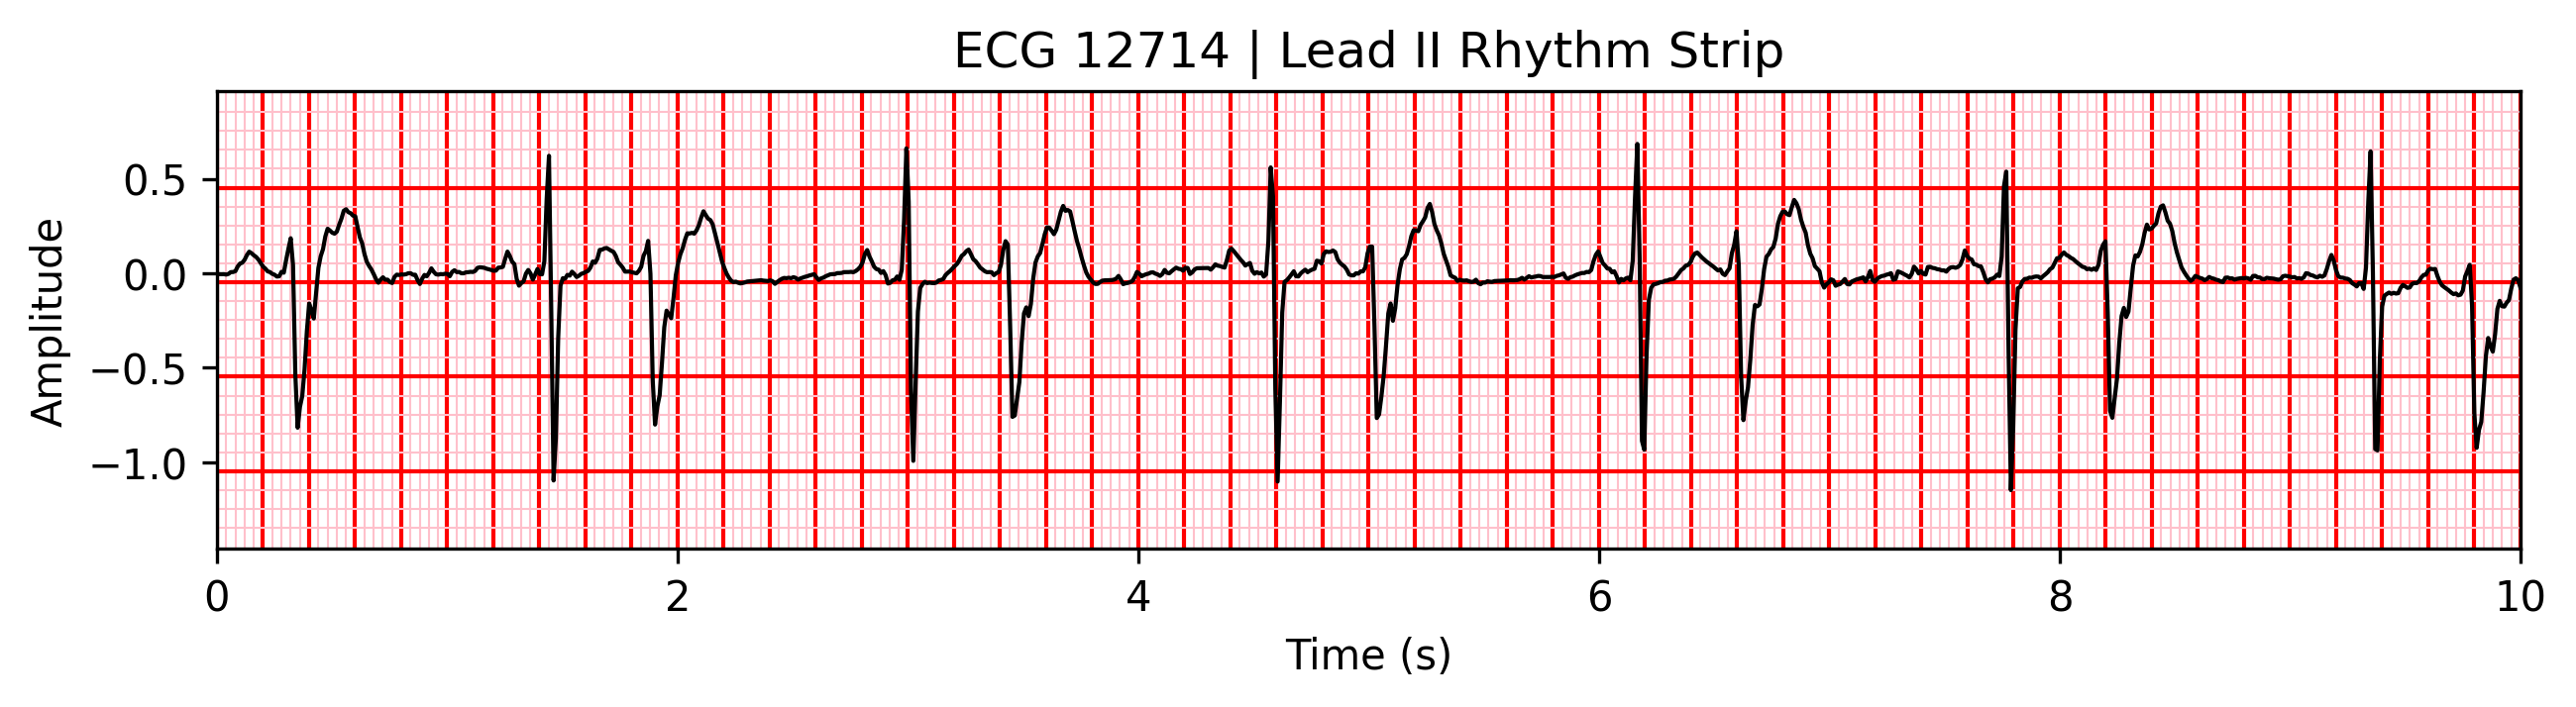
\includegraphics[width=0.7\linewidth]{images/prototype.png}
    \caption{Prototype learned for the BIGU class during training.}
    \label{fig:prototype}
\end{figure}

\begin{figure}[h]
    \centering
    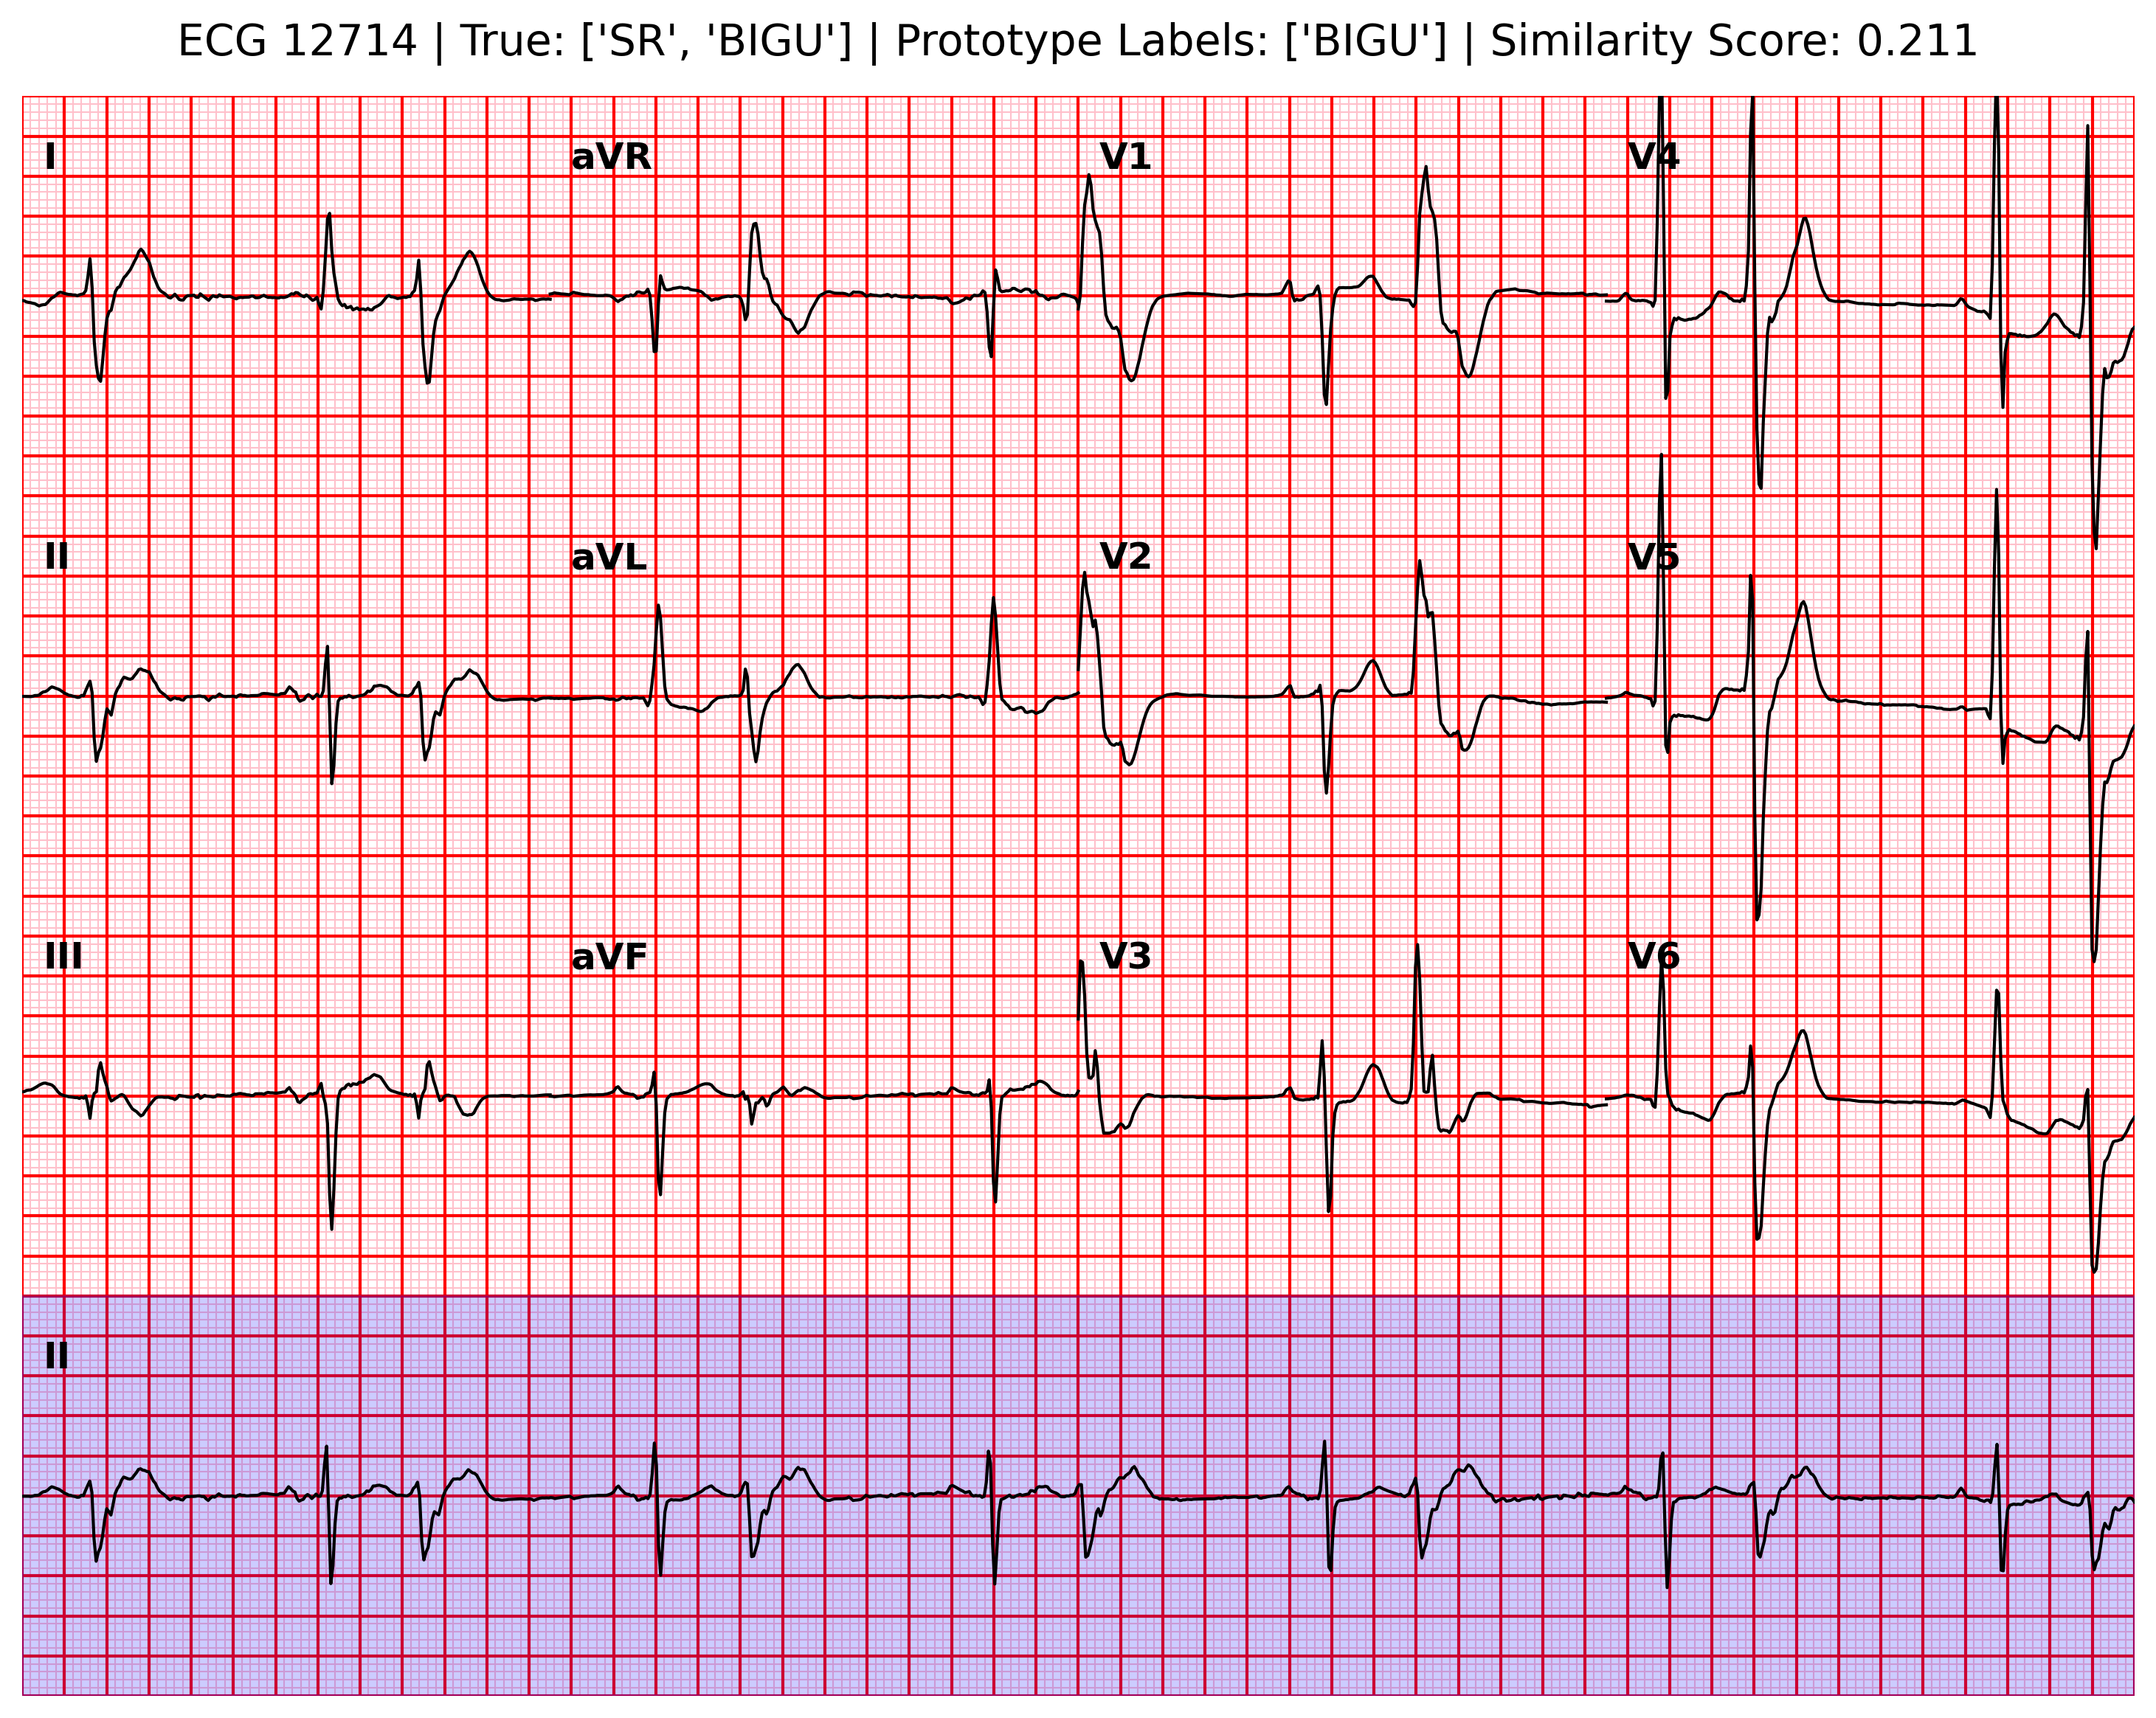
\includegraphics[width=0.7\linewidth]{images/full_ecg.png}
    \caption{Full ECG segment from which the BIGU prototype was extracted.}
    \label{fig:full_ecg}
\end{figure}

\section{Discussion}

Our findings show that prototype-based learning can deliver competitive performance on ECG rhythm classification tasks while preserving the critical advantage of interpretability. A key outcome is that joint training (optimizing both the feature extractor and the prototype layer together) is essential for this approach to succeed. The substantial performance difference between joint (0.8779 macro-AUROC) and separate training (0.5197 macro-AUROC) underscores the importance of learning representations that merge these two distinct steps in the learning process for the effective capture of the underlying patterns that allow to correctly diagnose cardiac abnormalities.

The model's clinical relevance is reinforced by its ability to maintain near-original performance (0.8779 vs. 0.8808) while substantially reducing computational demands. This makes it well-suited for deployment in constrained environments such as rural clinics or point-of-care settings with limited hardware capacity. Moreover, the interpretability offered by prototype-based models supports clinician trust by providing transparent, case-based explanations grounded in real ECG patterns.

Despite these promising results, the scope of our evaluation was limited to rhythm classification, which does not encompass the full complexity of ECG interpretation, such as morphological anomalies. Additionally, infrastructure constraints prevented us from conducting extensive hyperparameter tuning, a step the original ProtoECGNet paper performed using distributed optimization techniques. As such, our model may not represent the peak performance achievable with our simplified approach.

Our interpretability analysis, while indicative of meaningful prototype learning, was largely qualitative. The original study incorporated structured expert validation of prototype utility, which we could not replicate. A future direction for extending this work would be to formalize interpretability metrics and involve clinical stakeholders in prototype assessment.

Importantly, the original implementation of ProtoECGNet was both well-documented and reproducible, which played a crucial role in our ability to replicate key results and extend the work. This highlights a broader point about the value of reproducibility in scientific research software: accessible, transparent implementations are foundational for meaningful progress in clinical AI and should be treated as a standard rather than an exception.

Our results also offer a broader insight for clinical deployment strategies. The marginal performance trade-off from model simplification suggests a viable pathway for modular AI systems in healthcare. Rather than monolithic, multi-task models, a collection of focused, lightweight components could be deployed incrementally and tailored to specific diagnostic needs and resource environments. This strategy aligns well with clinical workflows and may lower the barrier to adoption in real-world practice.

\section{Conclusion}

This study demonstrates that a simplified prototype-based model can retain nearly all the diagnostic accuracy of a more complex system for ECG rhythm classification, while improving computational efficiency and preserving interpretability. Our key findings address three critical aspects of clinical AI deployment: performance, efficiency, and explainability.

\subsection{Research Question Responses}

\begin{itemize}
    \item \textbf{Performance: Can a simplified ProtoECGNet maintain competitive accuracy?} Our joint training approach achieves 0.8779 macro-AUROC, representing 99.7\% of the original model's rhythm classification performance while using significantly fewer computational resources.
    \item \textbf{Efficiency: Does simplification improve computational feasibility?} The rhythm-only architecture reduces model parameters by 60\% and training time by 70\%, making deployment viable in resource-constrained healthcare settings.
    \item \textbf{Interpretability: Do prototype-based explanations enhance clinical understanding?} The learned prototypes provide case-based reasoning that aligns with clinical diagnostic processes, offering transparent explanations for automated ECG rhythm classification decisions.
\end{itemize}

In addition to these contributions, our success in reproducing the original results emphasizes the value of reproducible and well-documented scientific software, particularly in medical AI research where trust, verification, and regulatory oversight are paramount.

Looking ahead, further work should expand this approach to include other ECG diagnostic categories, integrate automated hyperparameter optimization, and pursue rigorous validation of prototype interpretability through clinical partnerships. By continuing to prioritize accuracy, interpretability, and accessibility, we can help close the gap between research-grade AI models and tools that are viable in everyday clinical practice.


\bibliographystyle{ACM-Reference-Format}
% if your .bib file is not named references.bib then replace the name in the line below
\bibliography{references}
\newpage
\onecolumn
\newpage
\appendix

\begin{appendices}

\section{Extra figures}

\begin{figure}[h]
    \centering
    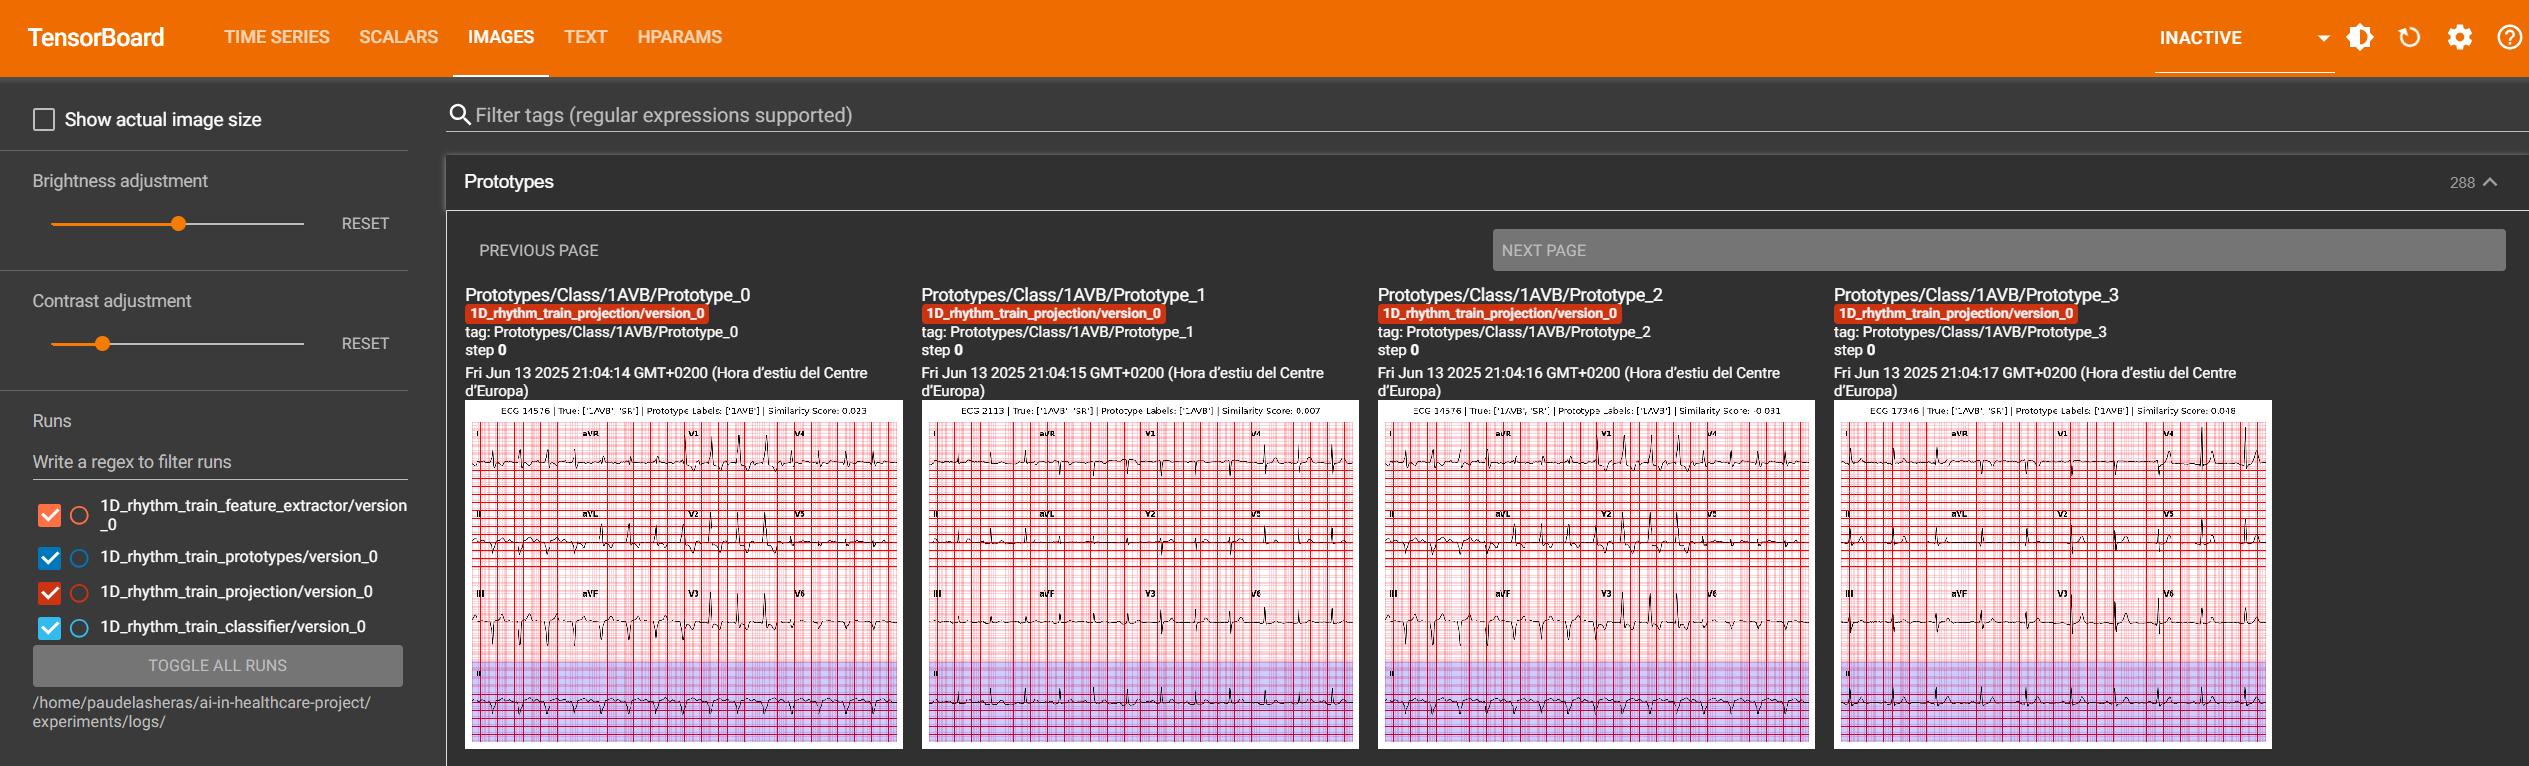
\includegraphics[width=0.9\linewidth]{images/tensorboard.png}
    \caption{Screenshot of TensorBoard used for prototype visualization and training monitoring.}
    \label{fig:tensorboard}
\end{figure}

\end{appendices}

\end{document}